%%%%%%%%%%%%%%%%%%%%%%%%%%%%%%%%%%%%%%%%%%%%%%%%%%%%%%%%%%%%%%%%%%%%%%%%%%%%%%%%
%%%                               80 COLONNES                                %%%
%%%%%%%%%%%%%%%%%%%%%%%%%%%%%%%%%%%%%%%%%%%%%%%%%%%%%%%%%%%%%%%%%%%%%%%%%%%%%%%%

\chapter{Conclusions et perspectives}
\label{ChConcluPerspec}

%%%%%%%%%%%%%%%%%%%%%%%%%%%%%%%%%%%%%%%%%%%%%%%%%%%%%%%%%%%%%%%%%%%%%%%%%%%%%

\section{Conclusions générales}
\label{SecConcluGene}

Les réseaux de capteurs sans-fil (WSN), et par extension de l'Internet des
Objets (IoT), constituent un domaine de recherche et de développement très
actif~; ceci s'accompagne du développement d'applications toujours plus
nombreuses de ces réseaux dans des domaines sans cesse plus variés.
Ce développement promet encore de s'accélérer avec l'évolution des
technologies et la montée en puissance des noeuds (\lang{``motes''})
constituant ces réseaux.

Ces réseaux ont des objectifs contradictoires~: la qualité de service
(QdS) d'une part, et d'autre part l'économie d'énergie pour prolonger
la durée de vie des \lang{``motes''} et surtout de leur batteries.
Pour atteindre ces objectifs contradictoires, de nombreux efforts de
recherche ont été menés au niveau de la couche MAC (niveau 2 OSI) de
la pile réseau, comme nous l'avons vu dans la première partie du
chapitre \ref{ChEtatArt} sur l'état de l'art. Le standard IEEE 802.15.4,
sur lequel repose la plupart des WSN actuels, propose lui-même ses propres
couches MAC (avec leurs limitations), et une extension du standard---
802.15.4e~--- se consacre à amener un nouveau protocole MAC nettement
plus performant et complexe.

Nous avons également vu que ces WSN disposaient de systèmes d'exploitation
dédiés. Ces plates-formes logicielles spécialisées ont fait l'objet d'une
revue critique lors de la seconde partie du chapitre \ref{ChEtatArt}.

La comparaison de ces deux états de l'art nous montre que les nombreux et
divers protocoles MAC issus de travaux de recherche n'ont que très rarement
fait l'objet d'implantations dans les systèmes d'exploitations dédiés
(ContikiMAC étant la seule exception notable). La problématique de cette
thèse a donc consisté à faire avancer l'implantation effective de protocoles
MAC innovants et performants dans ces OS dédiés, afin d'améliorer le facteur
limitant que représentent, à l'heure actuelle, les couches basses des piles
réseau pour capteurs sans-fil.

Du chapitre \ref{ChEtatArt}, nous avons tiré la conclusion que
l'implantation de protocoles MAC hautes performances nécessitait
des fonctionnalités de la part de la plate-forme logicielle fournissant
la pile réseau~: il s'agit principalement de fonctionnalités temps-réel,
permettant de respecter des délais très stricts pour nos implantations,
ce qui est nécessaire pour une synchronisation suffisamment précise
entre noeuds communicants, laquelle est cruciale pour les protocoles
récents basés en particulier sur le multiplexage temporel (TDMA).
Nous avons constaté que les plates-formes logicielles les plus employées
et connues (Tiny OS et Contiki) n'étaient pas en mesure de fournir de
telles fonctionnalités~; cela explique notamment pourquoi ces systèmes
ne proposent que des protocoles MAC basés sur la contention (CSMA),
car ils sont dans l'incapacité de supporter des protocoles basés
sur des paradigmes plus exigeants en respect de contraintes temporelles.

Les travaux de notre thèse nous ont ainsi amené à rechercher une plate-forme
logicielle adéquate au chapitre \ref{ChPFLogicielles}. Nous avons étudié
deux plates-formes spécialisées~: Contiki et RIOT OS. Ce chapitre décrit
notre point de vue sur les forces et faiblesses de ces dernières, et tout
particulièrement une analyse critique de leurs piles réseau. Nous avons
alors choisi la plate-forme fournissant les fonctionnalités nécessaires.
Notre choix s'est porté sur RIOT OS, qui parmi de nombreux autres avantages,
se montre accueillant et ouvert aux contributions extérieures. Tout en
contribuant activement à son déboguage, son évolution et son portage sur
le matériel que nous utilisions à l'époque, nous avons ainsi pu implanter
avec succès notre premier protocole, S-CoSenS, sous RIOT.

Une fois cette implantation de S-CoSenS prête, nous avons au chapitre
\ref{ChProtocolesMAC} d'abord testé son bon fonctionnement, puis comparé ses
performances avec ContikiMAC, principalement via des tests effectués par des
simulations sous Cooja (le simulateur de réseaux de capteurs sans-fil du
projet Contiki), mais aussi quelques tests limités sur matériel. Il ressort
de ces tests que notre implantation de S-CoSenS sous RIOT offre une
meilleure QdS que ContikiMAC dans son implantation standard sous Contiki,
tandis que ce dernier~--- si l'on se fie à l'indicateur certes imparfait que
sont les \lang{``duty cycles''}~--- obtient clairement de meilleurs
résultats concernant les économies d'énergie. Nous avons conclu de ces tests
que comme nous le pensions, des fonctionnalités temps-réel sont nécessaires
pour implanter des protocoles MAC novateurs et efficaces. Nous avons
également proposé des pistes pour faire face aux problèmes de corruption
mémoire en l'absence de mécanismes matériels de protection mémoire,
ainsi que plusieurs techniques susceptibles d'améliorer la robustesse
des protocoles MAC~/ RDC, grâce à une meilleure évaluation du trafic
réseau courant, et une adaptation dynamique du rapport signal~/
bruit (SNR).

La supériorité affichée du protocole S-CoSenS en matière de QdS, au
détriment du \lang{``duty cycle''}, correspond à notre approche~: nous
pensons en effet que la première priorité d'un WSN est de transmettre
correctement les données qui lui sont confiées (QdS), l'économie d'énergie
étant une seconde priorité, qui ne doit pas nuire à la première.
Nos tests montrent que le protocole S-CoSenS assure bien mieux le bon
ordre de ces priorités que ContikiMAC, spécialement quand le trafic
réseau est intense.

En testant l'influence de l'implantation des pilotes SPI des OS dédiés
sur les performances de communication, nous avons été amenés à découvrir
des inexactitudes importantes, au niveau temporel, dans les simulations
effectuées par Cooja. Nous avons alors étudié ce problème, et avons
détaillé nos découvertes au début du chapitre \ref{ChValidation}.
Nous avons déterminé que le problème venait de l'émulateur MSPSim,
que Cooja utilise pour émuler les matériels basés sur l'architecture
MSP430. Le problème vient visiblement d'un problème de calibration des
délais d'émulation du bus SPI, l'inexactitude de calibration variant
visiblement selon le microcontrôleur émulé. Il est par exemple clair
que si l'erreur de calibration reste modérée pour le MSP430F1611
équipant entre autres la TelosB~/ Skymote, elle devient extrêmement
gênante pour le MSP430F2617 équipant la Zolertia Z1.

Notre conclusion est que tant que ces erreurs de calibration ne sont
pas corrigées, les tests sur matériels sont seuls à même de permettre
des évaluations de performances fiables (approche empirique). Cooja
reste quoi qu'il en soit un outil très utile, notamment pour faciliter
le dévoppement et le déboguage d'applications sur capteurs sans-fil.

La suite de ce même chapitre détaille les travaux que nous avions prévus
d'effectuer sur du matériel réel pour valider nos expériences précédentes
concernant S-CoSenS, puis tester sa montée en charge, notamment en mettant
en oeuvre un réseau comportant de nombreux noeuds et divisé en différents
sous-réseaux, reproduisant ainsi plus fidèlement un <<~logement
intelligent~>> richement pourvu en appareils susceptibles d'appartenir
à un WSN. Nous avons choisi d'effectuer les dits travaux sur le
\lang{testbed} IoT-LAB, offrant l'accès à de très nombreuses \lang{motes},
dont les plus récentes (IoT-LAB M3) offrent une puissance confortable
et des possibilités d'instrumentation riches et avancées.

Malheureusement, seule la première partie de ces travaux a pu être menée
à terme, des problèmes techniques nombreux et complexes nous ayant empêché
de terminer leur réalisation. Nous avons toutefois validé notre idée
d'amélioration générique de l'API des pilotes radio, idée reprise par
Contiki et RIOT OS dans sa nouvelle pile réseau. Nous n'avons au final
pas pu réaliser et implanter toutes nos idées de tests et d'optimisations,
mais celles-ci peuvent servir de contributions pour des travaux
ultérieurs.

%%%%%%%%%%%%%%%%%%%%%%%%%%%%%%%%%%%%%%%%%%%%%%%%%%%%%%%%%%%%%%%%%%%%%%%%%%%%%

\section{Contributions de la thèse~: résumé}

Au final, les principales contributions de cette thèse sont les suivantes~:

\begin{itemize}

\item \emph{L'analyse des différentes plates-formes logicielles (systèmes
d'exploitation) dédiées aux réseaux de capteurs sans-fil, et de leurs
fonctionnalités} (section \vref{SecOSWSN} de l'état de l'art).

\item \emph{De nombreuses contributions techniques amenées au projet RIOT
OS} (section \vref{SecRIOTContrib})~: notamment l'ajout d'un mécanisme de
gestion des erreurs fatales, le portage du système sur la \lang{mote}
Zolertia Z1, et la résolution d'un problème majeur qui empêchait RIOT OS
de fonctionner de façon fiable sur les systèmes à architecture MSP430.
À cela peuvent s'ajouter de nombreuses autres contributions mineures
au projet RIOT, ainsi qu'une contribution partielle et indirecte au projet
Contiki (cf. section \vref{ParAPIRadioContiki}).

\item \emph{Nous nous sommes penchés sur la nouvelle pile réseau (<<~gnrc~>>)
de RIOT, montré ses possibilités et les améliorations qu'elle apporte,
ainsi que ses défauts} (section \vref{SecGnrcRIOT}). Nous sommes confiants
sur le fait qu'une fois ces derniers corrigés ou contournés \footnotemark[1],
RIOT OS deviendra une plate-forme encore plus performante et pratique
pour les réseaux de capteurs sans-fil.

\footnotetext[1]{Notamment par la conception d'une pile alternative plus
légère, dédiée aux appareils très limités et~/ ou aux applications
nécessitant des réactions extrêmement rapides aux évènements réseau
(sans passer par une pile complète et complexe).}

\item \emph{L'affirmation de l'utilité~--- et même de la nécessité~---
de fonctionnalités temps-réel avancées pour implanter des protocoles
MAC~/ RDC évolués}, offrant à la fois une qualité de service maximale
et une consommation d'énergie optimale (les \lang{``duty cycles''}
étant les marqueurs nous ayant été les plus accessibles, bien que très
imparfaits, pour appréhender cette consommation énergétique).
Une première démonstration en a été faite avec l'implantation de
S-CoSenS sous RIOT OS, et une comparaison avec ContikiMAC donnant des
résultats encourageants (en partie confirmée par des tests sur matériel),
\emph{particulièrement les bons résultats de S-CoSenS en termes de QdS
en présence d'un trafic réseau intense}. Cela correspond à l'approche
que nous avons revendiquée en conclusion du chapitre \ref{ChProtocolesMAC}
(section \vref{SecDiscussContribConcluProtocolesMAC}).

\item \emph{Plusieurs perspectives d'amélioration des couches basses des
piles réseau des plates-formes spécialisées dans les capteurs sans-fil},
idées dont la description et les bénéfices~/ contributions attendus sont
décrits en section \vref{SecAmeliorAlgoProtoMAC}.

\item \emph{La découverte et l'analyse d'un problème d'inexactitudes sévères
au niveau temporel~--- délais de communication entre microcontrôleur et
émetteur~/ récepteur radio~--- dans le simulateur de réseaux de capteurs
sans-fil Cooja} (ou plutôt~: dans l'émulateur MSPSim sur lequel il s'appuie).
Nous avons fourni des pistes sérieuses quant à la cause de cette anomalie~---
mauvaises calibrations des délais d'émulation, variables selon le MCU~---
dans l'espoir de faciliter sa future correction. Nous avons enfin tenté
d'analyser le retentissement de ce problème sur la validité des travaux
d'évaluation de performances réalisés grâce à cet outil~--- y compris
la validité de nos propres travaux de simulation précédents. Cette
contribution correspond à la section \vref{SecLimInexactSimu} constituant
la première partie du chapitre \ref{ChValidation}.

\item \emph{La validation de nos expériences réalisées par simulation~/
émulation grâce à des tests sur du matériel réel disposant des capacités
d'instrumentation adéquates}, tests décrits en \vref{SubsecTravauxValidPrevus}.
Malheureusement, seul le premier de ces travaux a pu être réalisé à cause
des problèmes techniques décrits en section \vref{SubsecPbTech}.
\emph{Nous avons alors donné tous les détails techniques en notre possession,
souhaitant aider à la résolution~--- dans des travaux ultérieurs~--- de ces
difficultés} dont les causes, visiblement complexes, restent actuellement
pour nous inconnues et incompréhensibles. Ceci constitue la seconde et
dernière partie du chapitre \ref{ChValidation}.

\end{itemize}

%%%%%%%%%%%%%%%%%%%%%%%%%%%%%%%%%%%%%%%%%%%%%%%%%%%%%%%%%%%%%%%%%%%%%%%%%%%%%

\section{Perspectives}
\label{SecPerspectives}


\subsection{Perspectives à court terme}
\label{SubsecPerspCourt}

Les perspectives à court terme consisteraient bien évidemment à terminer
les travaux prévus en section \vref{SubsecTravauxValidPrevus} du présent
manuscrit, pour confirmer (ou non) de façon indiscutable la validité des
expériences effectuées dans la présente thèse, pour lesquelles nous avons
majoritairement eu recours aux techniques de simulation~/ émulation.

Nous nous efforçons actuellement, avec le soutien actif de l'équipe de
développement de RIOT OS, d'adapter S-CoSenS à la nouvelle pile <<~gnrc~>>
de ce système, dans l'espoir d'obtenir ainsi des avancées, ou au moins
des informations complémentaires, concernant les problèmes qui nous ont
empêché de mener à leur terme nos travaux de validation.

\medskip

Dans un second temps, afin de compléter les solutions à la problématique
posée par la présente thèse, et d'en tirer de nombreux bénéfices et
contributions, il serait fort utile de procéder aux tests des améliorations
décrites en section \vref{SecAmeliorAlgoProtoMAC}. Nous pensons notamment à~:

\begin{itemize}

\item L'étude de l'influence des SFD sur S-CoSenS~;

\item L'étude plus largement de l'influence du SNR (comme le fait le
protocole AEDP présenté dans la section sus-citée) sur l'amélioration
de la couche MAC des piles réseau.

\end{itemize}

\medskip

Dans un troisième temps, nous pensons qu'il serait extrêmement profitable
de s'intéresser à l'implantation du protocole iQueue-MAC (voir section
\vref{PariQueueMAC} dans l'état de l'art), dont nous n'avons pas pu nous
occuper durant la présente thèse. Il s'agit de l'un des protocoles MAC~/
RDC parmi les plus performants disponibles actuellement, et l'un de nos
objectifs initiaux était notamment de mesurer ses performances en matière
de consommation d'énergie, grâce à l'instrumentation spécifique des noeuds
d'IoT-LAB.

Plus précisement, il se trouve qu'iQueue-MAC a déjà été testé sur
matériel \cite{iQueueMAC}, mais en dehors du cadre d'une plate-forme
logicielle. La contribution attendue de ces tests sur matériel est donc
de déterminer clairement \emph{l'influence d'une plate-forme comme RIOT OS,
multitâche et pourvue de fonctionnalités temps-réel avancées, sur les
performances d'un protocole évolué comme iQueue-MAC.}
L'implantation du protocole iQueue-MAC, plus avancé, au sein du système
RIOT OS, et son intégration dans la nouvelle pile réseau <<~gnrc~>> serait
ainsi une contribution majeure, permettant d'offrir à cette plate-forme
logicielle un protocole MAC~/ RDC très performant au sein de sa pile réseau.

Nous travaillons actuellement avec l'un des auteurs de ce protocole, S. Zhuo,
dans le cadre d'une collaboration pour tenter d'implanter et de tester nos
protocoles avancés~--- S-CoSenS et iQueue-MAC~--- sur RIOT et sa nouvelle
pile gnrc, en développant et testant directement sur une des plates-formes
matérielles de référence de RIOT OS~: la carte d'évaluation Atmel
SAMR21 Xplained Pro, contenant un MCU avec émetteur~/ récepteur radio
802.15.4 intégré. Cette collaboration, déjà évoquée à la fin de la section
\vref{SubsecEtatActuel}, avance progressivement, l'une des premières tâches
en cours de réalisation est de faire fonctionner la couche MAC IEEE 802.15.4
de base (sans \lang{``beacon''}). Différents tests sur matériel ont déjà
permis à S. Zhuo de valider le fonctionnement du module \texttt{csma\_sender}
que nous avons proposé pour la pile gnrc de RIOT (PR \#4178), comme le montre
la capture d'écran d'un \lang{``sniffer''} de paquets ayant capté une
transmission entre deux cartes SAMR21 en figure \vref{FigSnifferSAMR21}.
Quelques problèmes subsistent pour faire fonctionner la couche MAC 802.15.4
que nous avons proposée (PR \#4184), mais ce premier objectif semble
\lang{a priori} réalisable à court terme (dans les semaines qui viennent).
L'implantation de S-CoSenS, et \lang{a fortiori} iQueue-MAC, qui sont
des protocoles bien plus avancés et complexes, demandera sans doute
un délai plus long.

\begin{figure}[!hbt]
\centering
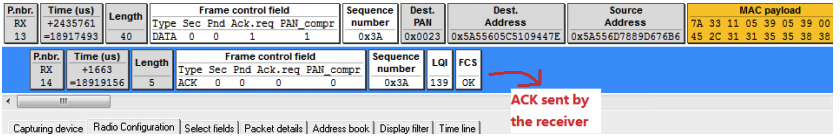
\includegraphics[width=12cm]{images/ch7-sniffer-SAMR21.png}
\flcaption{Capture d'écran d'un \lang{``sniffer''} de paquets Zigbee~/
802.15.4 lors de l'exécution de RIOT avec le module \texttt{csma\_sender}.
(Crédit~: Shuguo Zhuo, travail en cours.)}
\label{FigSnifferSAMR21}
\end{figure}

\medskip

En outre, il serait intéressant d'étudier le comportement de ce protocole
sur un réseau de topologie étendue (comme nous comptions le faire pour
parachever la validation de S-CoSenS). Tester l'influence de la variation
du \lang{``CCA Threshold''} (c'est-à-dire du SNR) sur ce protocole serait
sans doute également un test susceptible de fournir une contribution
intéressante.

\medskip

Enfin, un dernier test d'un grand intérêt serait notamment \emph{la 
comparaison d'iQueue-MAC avec la nouvelle couche MAC du standard amendé
IEEE 802.15.4e}~; cette dernière fait en effet appel au FDMA (changement
dynamique de canal, \lang{``channel hopping''}), ce que ne fait pas
iQueue-MAC, qui se propose plutôt d'utiliser un unique canal de la façon
la plus optimale possible. Le changement de fréquence étant une opération
nécessitant un certain délai (potentiellement long) durant lequel
l'émetteur~/ récepteur radio est indisponible, \emph{on peut légitimement
se demander lequel de ces deux protocoles MAC~/ RDC est le plus performant
en situation réelle. Une réponse claire à cette question serait une
contribution d'importance pour l'évolution des couches basses des piles
réseaux des WSN.}

\medskip

Tous ces tests seraient bien évidemment à réaliser, dans l'idéal,
sur du matériel en quantité suffisante, pourvu des fonctionnalités
d'instrumentation. L'une des plates-formes matérielles répondant à ces
exigences techniques serait le \lang{testbed} IoT-LAB. Cependant, comme
il l'a été dit en section \vref{SubsecEtatActuel}, résoudre les problèmes
techniques que nous avons rencontrés sur la plate-forme IoT-LAB, et
notamment ses noeuds M3, sera certainement un travail d'ingénierie et
de déboguage complexe, dont il est difficile d'estimer la durée
(probablement plusieurs mois si ces difficultés sont dues à plusieurs
causes combinées).


\subsection{Perspectives à long terme}
\label{SubsecPerspLong}

Les perspectives à long terme, en matière de réseaux de capteurs sans-fil,
sont immenses et semblent n'avoir comme limite que l'imagination.

\medskip

Concernant les couches basses des piles réseau des plates-formes logicielles
spécialisées dans les capteurs sans-fil, leur optimisation et surtout leur
fiabilisation devrait améliorer considérablement la qualité des liaisons
radio entre les \lang{motes} de ces réseaux, comme cette thèse a~---
nous espérons~--- commencé à le montrer.

\bigskip

Au cours de nos travaux, nous avons remarqué que les plates-formes
logicielles mais aussi et surtout matérielles semblent parfois peu adaptées,
et souffrent de limites pénalisantes. Si nous avons travaillé à
l'amélioration des plates-formes logicielles, nous voyons les limitations
suivantes aux plates-formes matérielles, lesquelles s'avèrent~--- nous le
pensons~--- inadaptées pour le développement futur de réseaux de capteurs
sans-fil à hautes performances~:

\begin{itemize}

\item Les limitations des microcontrôleurs (MCU). En la matière, le facteur
réellement limitant n'est pas la puissance de calcul, mais l'espace mémoire,
tout spécialement la RAM permettant de stocker les données, souvent
disponible en quantités trop faibles (10~Ko ou moins).\\
L'apparition de microcontrôleurs plus puissants (comme les Cortex-M
présents dans certains noeuds IoT-LAB) améliorent cet état de fait, mais
au prix d'une complexité nettement plus élevée~--- donc une programmation
et un déboguage plus délicats~--- que les architectures plus <<~classiques~>>
comme les MSP430 ou les AVR. En outre, le gain en puissance de calcul
apporté par ces nouveaux MCUs n'est souvent pas nécessaire, surtout
pour les noeuds-feuilles destinés surtout à interagir avec leur
environnement physique et non à faire des calculs complexes.

\item La séparation des émetteurs~/ récepteurs radio du MCU central~:
le programmeur d'une \lang{mote} se retrouve souvent à devoir programmer
deux puces principales, seul le MCU étant accessible au déboguage avancé
(en général via une liaison JTAG)~; la radio n'étant elle accessible
qu'indirectement~--- souvent par le bus SPI~---, il est donc difficile
de connaître précisément son état interne en cas de problème complexe
impliquant directement cette puce radio. (C'est l'une des difficultés
que nous avons rencontré au cours de nos travaux de déboguage que nous
avons détaillé en section \vref{ParDetailsTech}). \\
Bien sûr, un émetteur~/ récepteur radio séparé offre par contre l'avantage
d'être facilement interchangeable.

\end{itemize}

\bigskip

En fait, on peut réaliser qu'il n'existe encore que très peu de matériel
électronique \emph{spécifiquement} dédié aux capteurs sans-fil, les MCUs
étant des composants existant de longue date et souvent dédiés à des
applications embarquées aux besoins bien différents de ceux de nos
réseaux de capteurs sans-fil.

La situation commence à changer doucement, avec l'apparition de MCUs avec
radio intégrée, comportant en outre une quantité de RAM plus importante,
mieux adaptée aux travaux de développement sur capteurs sans-fil.
Un exemple récent est la famille Atmel AVR ATmegaRFR2 \cite{DSATmegaRFR2}
offrant, outre une radio intégrée comparable à celle équipant les noeuds
IoT-LAB M3, un espace mémoire allant jusqu'à 256~Ko de mémoire Flash
et 32~Ko de RAM, ce qui devient comparable aux MCUs plus complexes de
type ARM Cortex-M3. Outre cette mémoire accrue tout à fait bienvenue,
la présence de la radio directement sur le MCU rend les registres, et
donc le fonctionnement de cette radio, directement accessible aux sessions
de déboguage JTAG, facilitant grandement le travail du programmeur
d'applications pour réseaux de capteurs sans-fil (du moins pour les
noeuds n'ayant besoin que de cet unique émetteur~/ récepteur radio
intégré).

\medskip

Une solution matérielle commençant à être mise en {\oe}uvre est
d'utiliser des circuits logiques programmables~--- des \nom{FPGA}
(\lang{``Field-Programmable Gate Array''})~--- permettant de développer
des plates-formes matérielles parfaitement adaptées au rôle de capteur
sans-fil~: avec le choix de l'architecture processeur, de la quantité
de mémoire, voire même de l'émetteur~/ récepteur radio (si la technologie
le permet) optimaux pour une application donnée. Les FPGA devenant au
cours du temps de plus en plus vastes et de moins en moins chers, on peut
ainsi imaginer pouvoir développer un \lang{``System-on-Chip''} sur mesure
pour chaque type de réseaux de capteurs sans-fil ou même pour chaque
application, tout en rendant la programmation et le déboguage plus aisés~;
d'autant plus que les FPGA modernes offrent la possibilité de
modifier\footnotemark[2] à la volée leur logique matérielle, permettant
de changer d'architecture matérielle comme on change de programme sur un
microcontrôleur classique.

\footnotetext[2]{On parle alors de \emph{reconfiguration} plutôt que de
reprogrammation, car il s'agit de matériel et non de logiciel.}

Cela rejoint en tout cas les notions de SDN (\lang{``Software-Defined
Network''}) et de \lang{``Software-Defined Radio''}. De même, certaines
équipes de recherches et entreprises travaillent déjà sur des FPGA
dans des buts similaires. On peut notamment citer le projet NetFPGA
\cite{NetFPGA} déjà mature et largement utilisé\footnotemark[3].
\footnotetext[3]{Site Web~: \texttt{http://netfpga.org/}}

Peut-être s'agit-il là de l'avenir des réseaux de capteurs sans-fil,
voire même des systèmes embarqués dans leur ensemble~?


%%%%%%%%%%%%%%%%%%%%%%%%%%%%%%%%%%%%%%%%%%%%%%%%%%%%%%%%%%%%%%%%%%%%%%%%%%%%%
%%%             FIN DU CHAPITRE "CONCLUSIONS ET PERSPECTIVES"             %%%
%%%%%%%%%%%%%%%%%%%%%%%%%%%%%%%%%%%%%%%%%%%%%%%%%%%%%%%%%%%%%%%%%%%%%%%%%%%%%



